\documentclass[a4paper,preprint,review,12pt,authoryear]{elsarticle}

% -----------------------------------------------------------------------------
% Decision-aware FCA summaries for MoE placement -- research manuscript draft
% Target journal: Future Generation Computer Systems (Elsevier)
% IMPORTANT: empirical result fields are intentionally unfilled. Do not submit
% until the Colab trace experiment and the required multi-GPU validation have
% been executed and independently reproduced.
% -----------------------------------------------------------------------------

\usepackage[T1]{fontenc}
\usepackage[utf8]{inputenc}
\usepackage{lmodern}
\usepackage{microtype}
\usepackage{amsmath,amssymb,amsfonts,amsthm,mathtools,bm}
\usepackage{booktabs,tabularx,array,multirow}
\usepackage{graphicx}
\usepackage{float}
\usepackage{xcolor}
\usepackage{enumitem}
\usepackage{siunitx}
\usepackage{url}
\usepackage{hyperref}
\usepackage[nameinlink,noabbrev]{cleveref}
\usepackage{tikz}
\usetikzlibrary{arrows.meta,positioning,fit,calc,shapes.geometric,shapes.misc,backgrounds,decorations.pathreplacing}
\usepackage{algorithm}
\usepackage{algpseudocode}
\usepackage{listings}
\usepackage{threeparttable}
\usepackage{adjustbox}

\hypersetup{colorlinks=true,linkcolor=blue!55!black,citecolor=blue!55!black,urlcolor=blue!55!black}
\graphicspath{{figures/}}
\journal{Future Generation Computer Systems}

\newtheorem{definition}{Definition}
\newtheorem{proposition}{Proposition}
\newtheorem{lemma}{Lemma}
\newtheorem{corollary}{Corollary}
\newtheorem{assumption}{Assumption}
\newtheorem{remark}{Remark}
\newcommand{\E}{\mathbb{E}}
\newcommand{\R}{\mathbb{R}}
\newcommand{\N}{\mathbb{N}}
\newcommand{\Ccal}{\mathcal{C}}
\newcommand{\Wcal}{\mathcal{W}}
\newcommand{\Pcal}{\mathcal{P}}
\newcommand{\Dcal}{\mathcal{D}}
\newcommand{\Ical}{\mathcal{I}}
\newcommand{\PiSet}{\mathcal{A}}
\newcommand{\Reg}{\operatorname{Reg}}
\newcommand{\Bytes}{\operatorname{Bytes}}
\newcommand{\supp}{\operatorname{supp}}
\newcommand{\argmin}{\operatorname*{arg\,min}}
\newcommand{\argmax}{\operatorname*{arg\,max}}
\newcommand{\card}[1]{\left|#1\right|}
\newcommand{\pending}{\textcolor{red!75!black}{\textbf{pending}}}
\newcommand{\todo}[1]{\textcolor{red!75!black}{\textbf{[TO COMPLETE: #1]}}}
\newcommand{\method}{\textsc{DPCK}}
\newcommand{\fca}{\textsc{FCA}}
\newcommand{\topk}{\textsc{Top-}K}

\begin{document}

\begin{frontmatter}

\title{Decision-Aware FCA Summaries for Workload-Shift-Robust Mixture-of-Experts Placement}

\author{Anonymous authors}
\address{Submitted for anonymous review}

\begin{abstract}
Sparse mixture-of-experts (MoE) inference creates a placement problem in which the routing decisions made for each token induce communication among devices that host the selected experts. Placement methods based on expert frequencies or pairwise co-activation are attractive because they are inexpensive, but pairwise statistics do not in general determine higher-order, per-token destination sets. Conversely, a complete routing-pattern histogram preserves the information required by a static additive communication objective, but may be expensive to retain and inspect when traces are collected across layers, sessions, and workload families. This paper formulates a decision-aware use of formal concept analysis (FCA) for this setting. We explicitly do not claim that a complete concept lattice is intrinsically more compact or more informative than a routing hypergraph. Instead, we define a budgeted Decision-Preserving Concept Kernel (DPCK): a selected set of FCA-derived, overlapping routing descriptors used as features for predicting placement costs over a common finite action set. The selection objective is downstream placement regret under workload-shift episodes, subject to an explicit serialized-byte budget. We prove an exact sufficiency result for weighted route histograms under separable static costs, give a Top-3 parity construction showing that identical pairwise marginals can induce disjoint sets of optimal placements, and establish a conditional $2\epsilon$ decision-regret bound for uniformly accurate cost estimators. We specify a leakage-resistant evaluation protocol using real router traces from an open MoE model, a Google Colab T4 runtime for trace capture, and a Hugging Face Space as a reproducibility and inspection interface. The proposed evaluation compares DPCK with equal-byte pairwise, hyperedge, closed-itemset, generic kernel-concept, clustering, and task-aware baselines. No empirical performance result is claimed in this manuscript: the T4 trace-capture and multi-GPU experiments are specified but remain to be executed. This explicit separation between formal guarantees, planned measurements, and unvalidated systems hypotheses is intended to make the study falsifiable and reproducible.
\end{abstract}

\begin{graphicalabstract}
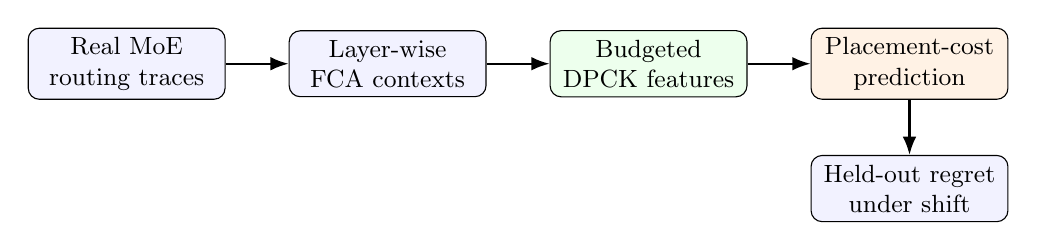
\begin{tikzpicture}[font=\small, node distance=7mm and 8mm, >=Latex,
  b/.style={draw,rounded corners,align=center,minimum height=8mm,minimum width=25mm,fill=blue!5},
  g/.style={draw,rounded corners,align=center,minimum height=8mm,minimum width=25mm,fill=green!7},
  o/.style={draw,rounded corners,align=center,minimum height=8mm,minimum width=25mm,fill=orange!10}]
  \node[b] (trace) {Real MoE\\routing traces};
  \node[b,right=of trace] (ctx) {Layer-wise\\FCA contexts};
  \node[g,right=of ctx] (kernel) {Budgeted\\DPCK features};
  \node[o,right=of kernel] (decision) {Placement-cost\\prediction};
  \node[b,below=of decision] (eval) {Held-out regret\\under shift};
  \draw[->,thick] (trace)--(ctx);
  \draw[->,thick] (ctx)--(kernel);
  \draw[->,thick] (kernel)--(decision);
  \draw[->,thick] (decision)--(eval);
\end{tikzpicture}
\end{graphicalabstract}

\begin{highlights}
\item Formalizes objective-specific sufficiency for static additive MoE placement.
\item Shows why pairwise routing marginals can fail for Top-3 destination costs.
\item Defines DPCK as a byte-budgeted, regret-driven selection of FCA features.
\item Separates T4 trace validation from physical multi-GPU systems evaluation.
\item Provides a preregisterable protocol and explicit empirical completion gates.
\end{highlights}

\begin{keyword}
Mixture-of-experts \sep expert placement \sep formal concept analysis \sep concept selection \sep workload shift \sep hypergraph \sep decision regret \sep distributed inference
\end{keyword}

\end{frontmatter}

% A visible warning is retained in the review draft so that unexecuted
% experiments cannot accidentally be mistaken for completed results.
\noindent\colorbox{yellow!25}{\parbox{0.97\linewidth}{\textbf{Manuscript status.} This is a complete methodological and experimental-protocol draft, not yet a submission-ready empirical article. The result tables deliberately contain pending markers. Replace them only with raw-data-backed results, confidence intervals, artifact identifiers, and logs. A single T4 cannot validate real multi-GPU all-to-all performance.}}

\section{Introduction}

Sparse mixture-of-experts models activate only a subset of their expert networks for each token. This conditional computation can increase model capacity without activating every parameter on every token, but it creates a systems problem: selected experts may reside on different accelerators, forcing token dispatch and result collection across device and network boundaries. The cost depends on the routing tuples, their source ranks, the expert-to-device mapping, and the execution topology.

A common strategy is to infer placement from expert activation frequencies or pairwise co-activation. This can be effective, but it is not universally sufficient. Recent work makes the workload dependence explicit: task-aware co-activation grouping derives different placement preferences from different task families and adds replication for experts that remain broadly useful across families \citep{xu2026tacg}. CAP uses co-activation-driven placement as one component of a broader communication--computation--accuracy trade-off \citep{shi2026cap}. These results create a high bar for a new representation: merely discovering that routing patterns differ across tasks is no longer a convincing contribution.

A related 2026 study formulates MoE distribution as a hypergraph-partitioning problem and evaluates replication on MoE-derived hypergraph benchmarks, reinforcing that exact route-set and replication-aware baselines are necessary rather than optional comparators \citep{papp2026replication}. The problem also falls within the broad FGCS interests in distributed dynamic resource management, high-performance computing, and large-scale communication and computation; this journal fit is strongest only after physical multi-GPU validation is completed \citep{fgcs2026scope}.

At the other end of the representation spectrum, a weighted histogram of complete routing tuples retains the observed higher-order combinations. For a static placement objective that is additive over routing events, this histogram is sufficient to evaluate every candidate placement exactly. Therefore, FCA cannot claim to contain more information than the exact route histogram. The relevant question is whether a selected set of FCA-derived descriptors can preserve placement decisions with lower storage or analysis cost, especially when a serving workload changes after the representation has been built.

This paper studies that narrower question. We use FCA to generate overlapping routing descriptors from layer-wise window contexts. A separate decision-aware selector, DPCK, retains a subset of those descriptors under a serialized-byte budget. A lightweight multi-output cost predictor maps the selected concept features to placement costs over a shared candidate action set. Selection is driven by validation regret across deployment episodes, not by concept support or lattice centrality alone.

We emphasize three boundaries. First, the full concept lattice is not asserted to be compact; lattice construction can be exponential in the context dimensions. Second, a concept extent is not automatically a disjoint workload regime. In our terminology, selected concepts are routing descriptors; a workload episode is defined by a separately specified temporal split. Third, a single-GPU T4 experiment can validate model instrumentation and offline placement-decision quality under an explicitly simulated topology, but it cannot demonstrate physical all-to-all latency, cross-rank contention, or multi-GPU load balancing.

\subsection{Research questions}

The study is organized around four falsifiable questions:
\begin{enumerate}[leftmargin=*,label=\textbf{RQ\arabic*:}]
  \item At equal serialized-byte budgets, does DPCK reduce held-out placement regret relative to support-ranked hyperedges, pairwise graphs, closed itemsets, generic kernel-concept selection, and clustering?
  \item Does any DPCK advantage persist when the workload mixture at deployment differs from the training mixture?
  \item Does the advantage persist across model precision, window size, activation threshold, and model architecture?
  \item When moved to a real expert-parallel runtime, do offline decision gains translate into lower measured communication and end-to-end latency after accounting for placement, replication, and reconfiguration costs?
\end{enumerate}

\subsection{Contributions and non-claims}

The intended contributions are:
\begin{itemize}[leftmargin=*]
  \item an objective-specific sufficiency formulation separating exact route information from approximate summaries;
  \item a constructive Top-3 counterexample showing the limitations of pairwise route marginals for a destination-deduplicated cost;
  \item a formal FCA feature representation and a byte-budgeted DPCK selection objective based on downstream placement regret;
  \item a conditional decision-regret guarantee for uniformly accurate placement-cost estimates;
  \item a leakage-resistant, equal-budget experimental protocol with T4 trace capture and a separate multi-GPU validation stage.
\end{itemize}

We do not claim that FCA is universally superior to hypergraphs, that concept lattices are inherently smaller than route histograms, that FCA concepts are semantic expert specializations, or that the planned T4 stage demonstrates distributed execution speedups.

\section{Background and related work}
\label{sec:related}

\subsection{MoE placement and task-conditioned routing}

Expert-parallel MoE serving dispatches token representations to the devices hosting the selected experts. Placement influences communication volume, computation balance, and potentially the replication or memory footprint of experts. TACG explicitly argues that a task-agnostic co-activation plan can average away task-family-specific structure; it builds task-family preferences and uses generic-expert shared replication to improve robustness to workload skew \citep{xu2026tacg}. CAP combines co-activation placement with computation--communication adjustment and communication-aware pruning, and reports throughput gains in its own single-node and multi-node setup \citep{shi2026cap}. These are direct systems competitors for the placement problem, and the proposed evaluation must compare against their relevant graph-based ideas rather than only against naive frequency placement.

The value of higher-order routing events is also relevant to graph partitioning with replication. Papp et al. analyze replication in graph partitioning and scheduling and show that replication can materially change communication costs and complexity \citep{papp2026replication}. Their work motivates treating replication as an explicit extension rather than silently folding it into a simple one-copy placement model.

\subsection{Trace-driven MoE serving}

MoE-Infinity uses request-level activation traces to guide expert prefetching and caching for offloaded serving \citep{xue2024moeinfinity}. ExpertFlow combines routing-path prediction, expert caching, and token scheduling \citep{he2026expertflow}. These systems establish that routing traces already support predictive serving mechanisms. The present paper does not claim caching or prefetching as its primary contribution; it focuses on decision-aware pattern summaries for static placement epochs. Any future caching extension would need to compare against sequence-aware predictors and cache-management systems, not merely LRU.

\subsection{FCA and concept-kernel selection}

FCA represents a binary relation through formal concepts, each comprising an extent and an intent, ordered into a complete lattice \citep{ganter1999fca}. The intents of formal concepts are exactly the closed itemsets of the corresponding formal context. Thus a closed-itemset miner is not a different information model when it operates on the same transactions and attributes; it is an alternative mining and selection implementation.

Alwersh and Kov\'acs introduced the Kernel Concept Set (KCS) approach for selecting concepts using a derivation-cost function and frequency/structural criteria \citep{alwersh2024kcs}. Kov\'acs and Alwersh later studied kernel-concept mining with optimization of concept-set generation costs \citep{kovacs2026kernel}. These are direct methodological baselines. DPCK differs only if its selected set is optimized for downstream placement regret under distribution shift and an explicit byte budget. This distinction must be established experimentally, not inferred from different terminology.

\subsection{Positioning}

The proposed method does not replace an exact hypergraph. It tests whether a selected feature map over FCA-derived concepts can act as a compact decision interface. The full route histogram remains the exact reference for static additive costs; the pairwise graph, top-frequency hyperedges, closed-itemset selection, KCS, clustering, and task-aware grouping are competing summaries.

\section{Problem formulation}
\label{sec:problem}

\subsection{Routing events and placements}

Let $\mathcal{L}$ denote the set of MoE layers, $E_\ell$ the experts in layer $\ell$, and $\mathcal{D}$ the set of devices. A routing event is
\begin{equation}
 r_t=(\ell_t,s_t,R_t,w_t,\tau_t),
 \label{eq:event}
\end{equation}
where $\ell_t\in\mathcal{L}$ is the layer, $s_t\in\mathcal{D}$ is the source device/rank, $R_t\subseteq E_{\ell_t}$ is the exact selected expert set, $w_t$ identifies a window/session, and $\tau_t$ is an event-order key. For a fixed router with Top-$K$, $|R_t|=K$ unless the architecture or masking mechanism specifies otherwise.

A non-replicated placement is a mapping $\pi_\ell:E_\ell\rightarrow\mathcal{D}$. Feasibility is constrained by per-device expert memory:
\begin{equation}
 \sum_{e:\pi_\ell(e)=d}m_{\ell,e}\le C_d,\qquad \forall d\in\mathcal{D},
 \label{eq:capacity}
\end{equation}
where $m_{\ell,e}$ is expert memory and $C_d$ is the device capacity allocated to experts. Let $\PiSet$ be a finite, shared candidate set of feasible placements generated before comparing summary methods. Every method must use the same $\PiSet$ and the same placement-cost evaluator.

For destination-deduplicated dispatch, define
\begin{equation}
 D(R_t,\pi,s_t)=\{\pi_{\ell_t}(e):e\in R_t,\ \pi_{\ell_t}(e)\ne s_t\}.
\end{equation}
The primary offline cost in the first study is the number of distinct remote destination devices contacted by the token:
\begin{equation}
 c(r_t,\pi)=\card{D(R_t,\pi,s_t)}.
 \label{eq:tokencost}
\end{equation}
This is a trace-level proxy for destination fan-out. It is not a measurement of network bytes, all-to-all completion time, or contention. A hardware-aware extension may replace it with $b_t\sum_{d\in D}\delta(s_t,d)$, where $b_t$ is payload bytes and $\delta$ is a topology-dependent link cost; the extension must be calibrated and validated on real hardware.

For a trace multiset $\Dcal$, the static additive objective is
\begin{equation}
 J(\pi;\Dcal)=\sum_{r_t\in\Dcal}c(r_t,\pi),\qquad
 \pi^*(\Dcal)=\argmin_{\pi\in\PiSet}J(\pi;\Dcal).
 \label{eq:objective}
\end{equation}
When ties occur, use a deterministic tie-breaking rule fixed before evaluation.

\subsection{Weighted route histogram sufficiency}

\begin{definition}[Weighted route histogram]
For each layer, source, and exact route set, define
\begin{equation}
 H_{\ell,s}(R)=\sum_{t}\mathbf{1}[\ell_t=\ell,\ s_t=s,\ R_t=R].
 \label{eq:hist}
\end{equation}
\end{definition}

\begin{proposition}[Exact sufficiency for separable static cost]
\label{prop:suff}
Suppose the placement objective is separable over routing events and the per-event cost depends on an event only through $(\ell,s,R)$ and the placement. Then the weighted route histogram $H$ is sufficient to evaluate the objective exactly for every feasible placement:
\begin{equation}
 J(\pi;\Dcal)=\sum_{\ell,s,R}H_{\ell,s}(R)c(\ell,s,R,\pi).
 \label{eq:suff}
\end{equation}
Consequently, two traces with the same weighted route histogram have identical objective values for every $\pi\in\PiSet$ and identical optimal-placement sets.
\end{proposition}

\begin{proof}
Group the event-wise sum in \cref{eq:objective} by the equivalence classes $(\ell_t,s_t,R_t)$. Every event in one class has the same cost under a fixed placement by assumption. The number of events in that class is exactly $H_{\ell,s}(R)$. Summing class counts times class costs gives \cref{eq:suff}. Equal histograms therefore imply equal objective values pointwise over $\PiSet$, which implies equality of argmin sets.
\end{proof}

\begin{remark}
The proposition is deliberately scoped to static, event-separable costs. Queueing, concurrency, temporal dependencies, communication overlap, and time-dependent reconfiguration costs may require ordered batches or richer state. A route histogram is not claimed to be sufficient for those objectives.
\end{remark}

\subsection{Why pairwise marginals can be insufficient}

\begin{proposition}[Pairwise-equivalent Top-3 traces can have disjoint optimal placements]
\label{prop:parity}
Consider six experts $A_0,A_1,B_0,B_1,C_0,C_1$, three labelled devices with capacities $(3,2,1)$, a token source on device $1$, and the cost in \cref{eq:tokencost}. Let trace $\Dcal_{\mathrm{even}}$ contain the four equally weighted routes
\begin{equation*}
 \{A_0B_0C_0,\ A_0B_1C_1,\ A_1B_0C_1,\ A_1B_1C_0\},
\end{equation*}
and $\Dcal_{\mathrm{odd}}$ contain
\begin{equation*}
 \{A_0B_0C_1,\ A_0B_1C_0,\ A_1B_0C_0,\ A_1B_1C_1\}.
\end{equation*}
The traces have identical expert marginals and identical pairwise co-activation counts, yet their optimal-placement sets are disjoint. Exhaustive enumeration of the $6!/(3!2!1!)=60$ capacity-feasible labelled placements yields 12 optimal placements for each trace, each with mean cost $1.25$, and no placement is optimal for both. Applying an even-trace optimal placement to the odd trace yields mean cost $1.50$.
\end{proposition}

\begin{proof}
Each expert appears in exactly two of the four routes in either trace. For every cross-group pair, such as $(A_i,B_j)$, each of the four combinations appears exactly once in both traces; within-group pairs never co-occur. Hence all first- and second-order marginals agree. The placement claim follows by enumerating the 60 assignments satisfying the capacity vector and evaluating the four route costs under \cref{eq:tokencost}. The enumeration is also included as an executable unit test in the accompanying artifact. The proof is constructive and does not claim that pairwise summaries fail for every placement objective.
\end{proof}

\begin{figure}[H]
\centering
\resizebox{\linewidth}{!}{%
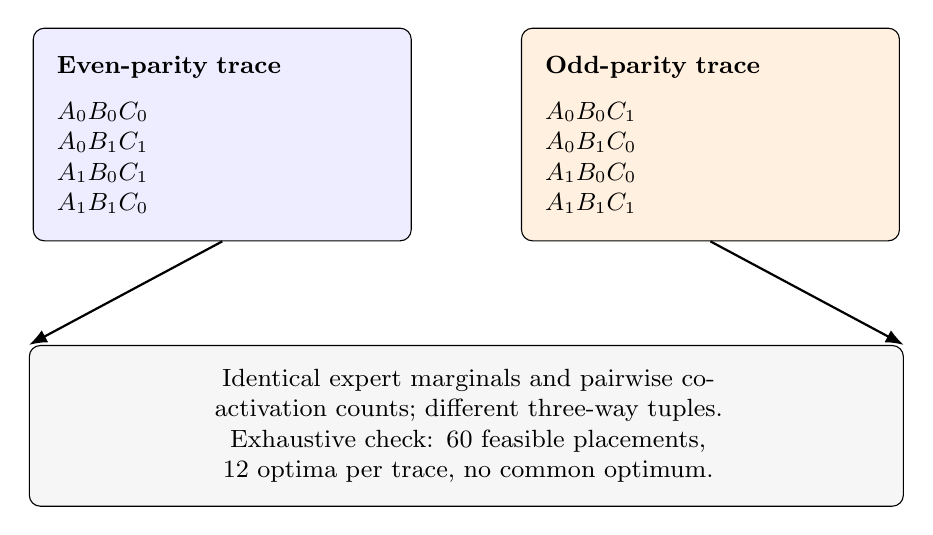
\begin{tikzpicture}[font=\small, >=Latex,
  routebox/.style={draw,rounded corners,align=left,text width=42mm,minimum height=27mm,inner sep=3mm},
  even/.style={routebox,fill=blue!7}, odd/.style={routebox,fill=orange!12},
  note/.style={draw,rounded corners,fill=gray!7,align=center,text width=105mm,minimum height=12mm,inner sep=3mm}]
  \node[even] (ev) at (0,0.15) {\textbf{Even-parity trace}\\[2mm]
    $A_0B_0C_0$\\$A_0B_1C_1$\\$A_1B_0C_1$\\$A_1B_1C_0$};
  \node[odd] (od) at (6.2,0.15) {\textbf{Odd-parity trace}\\[2mm]
    $A_0B_0C_1$\\$A_0B_1C_0$\\$A_1B_0C_0$\\$A_1B_1C_1$};
  \node[note] (res) at (3.1,-3.55) {Identical expert marginals and pairwise co-activation counts; different three-way tuples.\\
    Exhaustive check: 60 feasible placements, 12 optima per trace, no common optimum.};
  \draw[->,thick] (ev.south) -- (res.north west);
  \draw[->,thick] (od.south) -- (res.north east);
\end{tikzpicture}%
}
\caption{A parity construction showing why pairwise co-activation can discard decision-relevant higher-order routing structure for a Top-3 destination-deduplicated objective. The placement counts are from exhaustive enumeration of the stated finite example, not from GPU measurements.}
\label{fig:parity}
\end{figure}

\section{FCA-derived routing descriptors}
\label{sec:fca}

\subsection{Layer-wise window contexts}

Let $\Wcal$ be a set of non-overlapping, fixed-token-count trace windows, constructed within sessions without crossing session boundaries. A final incomplete window is either dropped or explicitly token-weighted; the selected policy is fixed before analysis. For window $w$, layer $\ell$, and expert $e\in E_\ell$, define the activation rate
\begin{equation}
 q_{w,\ell,e}=\frac{1}{N_{w,\ell}}\sum_{t\in w:\ell_t=\ell}\mathbf{1}[e\in R_t],
 \label{eq:rate}
\end{equation}
where $N_{w,\ell}$ is the number of routed tokens observed at layer $\ell$ in window $w$. The binary context at threshold $\theta$ is
\begin{equation}
 I_{\theta,\ell}(w,e)=\mathbf{1}[q_{w,\ell,e}\ge\theta].
 \label{eq:context}
\end{equation}
Quantitative rates $q_{w,\ell,e}$ are retained as side information for diagnostic analyses; they are not silently reconstructed from the binary context. Separate layer-wise contexts avoid conflating expert identifiers across layers and permit layer-specific mining budgets.

\begin{definition}[Formal context and derivation]
For each layer, $K_\ell=(\Wcal,E_\ell,I_{\theta,\ell})$ is a formal context. For $X\subseteq\Wcal$ and $Y\subseteq E_\ell$, define
\begin{align}
 X'&=\{e\in E_\ell:\forall w\in X,\ I_{\theta,\ell}(w,e)=1\},\\
 Y'&=\{w\in\Wcal:\forall e\in Y,\ I_{\theta,\ell}(w,e)=1\}.
\end{align}
A formal concept is $(A,B)$ with $A'=B$ and $B'=A$. Its extent is $A$ and its intent is $B$.
\end{definition}

Concepts are ordered by extent inclusion (equivalently, reverse intent inclusion). The concept intents are closed itemsets of the same window--expert transaction context. This equivalence is a central baseline constraint: comparing DPCK only with a naive FCA implementation would not establish an FCA-specific advantage.

\subsection{Concept matching for unseen windows}

For a new window $w$, let $X_{w,\ell}=\{e:I_{\theta,\ell}(w,e)=1\}$. A selected concept $c=(A_c,B_c)$ matches when
\begin{equation}
 z_c(w)=\mathbf{1}[B_c\subseteq X_{w,\ell(c)}]=1.
 \label{eq:feature}
\end{equation}
The selected concept feature vector is $\bm z_S(w)=(z_c(w))_{c\in S}$. It is intentionally allowed to be multi-hot: concept extents and matching intents may overlap. No claim is made that concepts partition windows or constitute semantic task labels.

\begin{figure}[H]
\centering
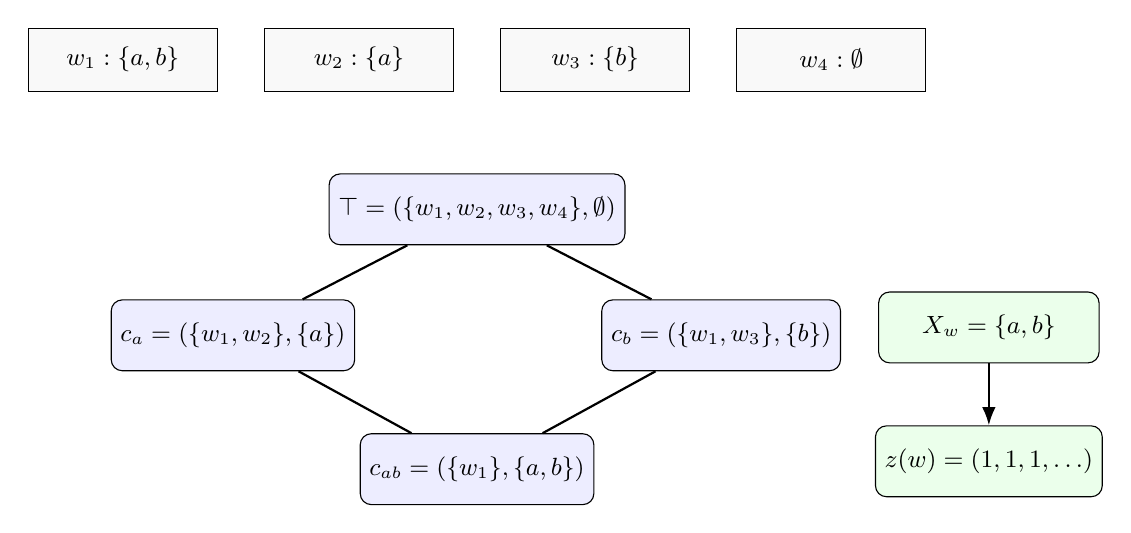
\begin{tikzpicture}[>=Latex, every node/.style={font=\small},
  cnode/.style={draw,rounded corners,minimum width=26mm,minimum height=9mm,align=center,fill=blue!7},
  onode/.style={draw,rounded corners,minimum width=28mm,minimum height=9mm,align=center,fill=green!8}]
  \node[draw,fill=gray!5,minimum width=24mm,minimum height=8mm] (w1) at (0,2.2) {$w_1:\{a,b\}$};
  \node[draw,fill=gray!5,minimum width=24mm,minimum height=8mm] (w2) at (3,2.2) {$w_2:\{a\}$};
  \node[draw,fill=gray!5,minimum width=24mm,minimum height=8mm] (w3) at (6,2.2) {$w_3:\{b\}$};
  \node[draw,fill=gray!5,minimum width=24mm,minimum height=8mm] (w4) at (9,2.2) {$w_4:\emptyset$};
  \node[cnode] (top) at (4.5,0.3) {$\top=(\{w_1,w_2,w_3,w_4\},\emptyset)$};
  \node[cnode] (a) at (1.4,-1.3) {$c_a=(\{w_1,w_2\},\{a\})$};
  \node[cnode] (b) at (7.6,-1.3) {$c_b=(\{w_1,w_3\},\{b\})$};
  \node[cnode] (ab) at (4.5,-3.0) {$c_{ab}=(\{w_1\},\{a,b\})$};
  \draw[thick] (top)--(a); \draw[thick] (top)--(b);
  \draw[thick] (a)--(ab); \draw[thick] (b)--(ab);
  \node[onode] (query) at (11.0,-1.2) {$X_w=\{a,b\}$};
  \node[onode] (feat) at (11.0,-2.9) {$z(w)=(1,1,1,\ldots)$};
  \draw[->,thick] (query)--(feat);
\end{tikzpicture}
\caption{A small formal context and its four-concept diamond lattice. The example illustrates that a window can match multiple concepts; the resulting feature vector is not a partition assignment.}
\label{fig:lattice}
\end{figure}

\subsection{Mining and truncation}

The number of formal concepts can be exponential in the size of the context. We therefore distinguish (i) the mathematical full lattice and (ii) the finite candidate pool $\Ccal_0$ actually made available to DPCK. The implementation will use a declared closed-itemset/concept miner with minimum support $\sigma$, maximum candidate count $C_{\max}$, and deterministic tie breaking. Every run must record whether enumeration completed, how many concepts were visited, the stopping reason, and the miner version. A truncated candidate pool is not reported as a complete lattice.

The primary analysis will quantify sensitivity to $\theta$, $\sigma$, window length, and $C_{\max}$. Exact concept stability is not required because its computation can be intractable; bootstrap recurrence and held-out feature stability are reported as empirical descriptors, not as exact FCA stability values.

\section{Decision-Preserving Concept Kernel}
\label{sec:dpck}

\subsection{A finite action-set cost predictor}

Let $\PiSet=\{\pi_1,\ldots,\pi_P\}$ be the fixed candidate placement set. For each training window $w$, calculate its exact per-routed-token placement-cost target vector from its route events:
\begin{equation}
 \bm y(w)=\big(J(\pi_1;\Dcal_w)/N_w,\ldots,J(\pi_P;\Dcal_w)/N_w\big)^\top.
\end{equation}
The concept features are mapped to predicted per-routed-token candidate costs using a multi-output linear predictor:
\begin{equation}
 \widehat{\bm y}_{S}(w)=\bm b+W\bm z_S(w).
 \label{eq:predictor}
\end{equation}
The linear predictor is chosen as a transparent baseline, not because linearity is assumed to be universally adequate. Ridge regularization is fitted within the training partition. A nonlinear predictor may be evaluated only as a separate ablation and must have its serialized parameters included in the budget.

For a deployment calibration prefix $C$ consisting only of windows observed before the placement decision, estimate the cost of each candidate placement by
\begin{equation}
 \widehat J_{S}(\pi;C)=\frac{\sum_{w\in C}N_w\widehat y_{S,\pi}(w)}{\sum_{w\in C}N_w},
 \qquad
 \widehat\pi_S(C)=\argmin_{\pi\in\PiSet}\widehat J_S(\pi;C).
 \label{eq:deployment}
\end{equation}
The selected placement is then evaluated on a later evaluation tail that is never used to construct the calibration prefix or select the kernel. This calibration/evaluation split defines the decision time and blocks future leakage.

\subsection{Budgeted selection objective}

A summary budget is measured in serialized bytes, not merely in the number of concepts. Let $\Bytes(S,W,\bm b)$ include the encoded expert intents, layer identifiers, feature metadata, predictor coefficients, intercepts, and required normalization constants. Training-only objects such as validation traces and the full lattice are excluded from the deployed artifact but their sizes and build costs are reported separately.

A deployment episode $q$ contains a calibration prefix $C_q$ and a later evaluation tail $T_q$. The reference placement is computed from the exact route histogram of $T_q$:
\begin{equation}
 \pi_q^*=\argmin_{\pi\in\PiSet}J(\pi;\Dcal_{T_q}).
\end{equation}
The regret of a summary is
\begin{equation}
 \Reg_q(S)=J(\widehat\pi_S(C_q);\Dcal_{T_q})-J(\pi_q^*;\Dcal_{T_q}).
 \label{eq:regret}
\end{equation}
The exact tail optimum is an offline evaluation oracle; it is not available to the serving system at decision time. If the solver cannot certify optimality, the manuscript must use the term \emph{best-known reference} and report the solver gap instead of calling it an optimum.

DPCK is defined as
\begin{equation}
 \begin{aligned}
 (S^*,W^*,\bm b^*)\in\argmin_{S,W,\bm b}\quad&
 \sum_{q\in\mathcal Q_{\mathrm{val}}}\omega_q\Reg_q(S,W,\bm b)\\
 \text{subject to}\quad&\Bytes(S,W,\bm b)\le B,\\
 &S\subseteq\Ccal_0.
 \end{aligned}
 \label{eq:dpck}
\end{equation}
Here $\omega_q$ is fixed before evaluation. Validation episodes cover the prespecified workload-mixture and shift scenarios. Workload-family labels may be used to stratify splits and define stress tests, but they are not passed as features to the label-free DPCK predictor.

\subsection{Selection algorithm}

The initial implementation uses byte-aware forward selection. At each iteration, it evaluates candidate concepts by the reduction in validation regret per incremental serialized byte, refits the predictor on training data, and selects the candidate with the best score. It stops when no candidate fits the remaining budget or no candidate improves validation regret by the prespecified minimum amount. This is a heuristic; no greedy approximation ratio is claimed. The exact selection problem can be combinatorial and the regret objective is not assumed to be monotone or submodular.

\begin{algorithm}[t]
\caption{Budgeted DPCK forward selection}
\label{alg:dpck}
\begin{algorithmic}[1]
\Require Candidate concepts $\Ccal_0$, training windows $\Wcal_{\rm tr}$, validation episodes $\mathcal Q_{\rm val}$, byte budget $B$, ridge parameter $\lambda$, minimum improvement $\delta$
\Ensure Selected kernel $S$ and fitted predictor $(W,\bm b)$
\State $S\gets\emptyset$; $b_0\gets\Bytes(\emptyset)$
\State Fit the intercept-only predictor and compute validation regret $R_0$
\While{there exists an unselected candidate fitting the remaining budget}
  \State $c^*\gets\bot$; $g^*\gets 0$
  \ForAll{$c\in\Ccal_0\setminus S$}
    \State $S'\gets S\cup\{c\}$
    \If{$\Bytes(S')\le B$}
      \State Fit $(W',\bm b')$ on $\Wcal_{\rm tr}$ using ridge regression
      \State $R'\gets$ mean validation regret of $(S',W',\bm b')$
      \State $g\gets (R_{S}-R')/[\Bytes(S')-\Bytes(S)]$
      \If{$g>g^*$} $c^*\gets c$; $g^*\gets g$; save $R'$, $W'$, $\bm b'$ \EndIf
    \EndIf
  \EndFor
  \If{$c^*=\bot$ or $R_S-R_{S\cup\{c^*\}}<\delta$} \State \textbf{break} \EndIf
  \State $S\gets S\cup\{c^*\}$; update saved predictor and regret
\EndWhile
\State \Return $S,W,\bm b$
\end{algorithmic}
\end{algorithm}

\subsection{Conditional decision-regret guarantee}

\begin{assumption}[Uniform cost-estimation accuracy]
For a fixed deployment distribution $Q$ and finite action set $\PiSet$, suppose the predictor induced by selected kernel $S$ satisfies
\begin{equation}
 \sup_{\pi\in\PiSet}|\widehat J_S(\pi;Q)-J(\pi;Q)|\le\epsilon.
 \label{eq:uniform}
\end{equation}
\end{assumption}

\begin{proposition}[Two-sided argmin stability]
\label{prop:2eps}
Under the preceding assumption, if $\widehat\pi_S\in\argmin_{\pi\in\PiSet}\widehat J_S(\pi;Q)$ and $\pi^*\in\argmin_{\pi\in\PiSet}J(\pi;Q)$, then
\begin{equation}
 J(\widehat\pi_S;Q)-J(\pi^*;Q)\le 2\epsilon.
\end{equation}
\end{proposition}

\begin{proof}
By uniform accuracy, $J(\widehat\pi_S;Q)\le\widehat J_S(\widehat\pi_S;Q)+\epsilon$. By estimated optimality, $\widehat J_S(\widehat\pi_S;Q)\le\widehat J_S(\pi^*;Q)$. Again by uniform accuracy, $\widehat J_S(\pi^*;Q)\le J(\pi^*;Q)+\epsilon$. Combining the inequalities yields the result.
\end{proof}

\begin{remark}
The bound is conditional on a uniform error guarantee and does not establish that FCA or DPCK achieves such a guarantee. Establishing useful error bounds from finite trace samples, particularly under distribution shift, is an empirical and statistical problem addressed by the evaluation protocol. The guarantee is representation-agnostic: the novelty question is whether FCA-derived features achieve a favorable error--byte trade-off relative to competing summaries.
\end{remark}

\section{Experimental methodology}
\label{sec:method}

\subsection{Two-stage evidence strategy}

The evaluation is deliberately divided into two stages. Stage A uses a single NVIDIA T4 runtime to verify model instrumentation, collect real router traces, and test offline placement-decision quality under declared simulated topologies. Stage B uses a real expert-parallel multi-GPU runtime to measure physical communication and latency. Stage A cannot substitute for Stage B.

\begin{figure}[H]
\centering
\resizebox{\linewidth}{!}{%
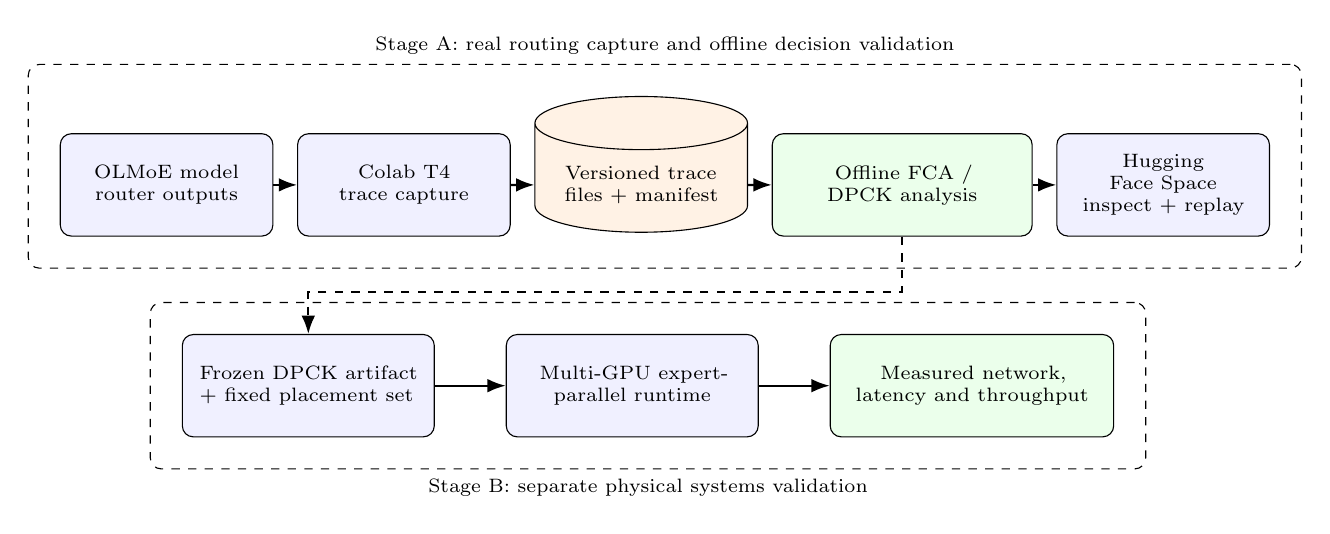
\begin{tikzpicture}[>=Latex, font=\scriptsize, node distance=3mm and 3mm,
  proc/.style={draw,rounded corners,fill=blue!6,align=center,text width=23mm,minimum height=13mm,inner sep=2mm},
  store/.style={draw,cylinder,shape border rotate=90,aspect=0.25,fill=orange!10,align=center,text width=23mm,minimum height=13mm,inner sep=2mm},
  eval/.style={draw,rounded corners,fill=green!8,align=center,text width=29mm,minimum height=13mm,inner sep=2mm}]
  \node[proc] (model) {OLMoE model\\router outputs};
  \node[proc,right=of model] (capture) {Colab T4\\trace capture};
  \node[store,right=of capture] (store) {Versioned trace\\files + manifest};
  \node[eval,right=of store] (analysis) {Offline FCA /\\DPCK analysis};
  \node[proc,right=of analysis] (space) {Hugging Face Space\\inspect + replay};
  \draw[->,thick] (model)--(capture);
  \draw[->,thick] (capture)--(store);
  \draw[->,thick] (store)--(analysis);
  \draw[->,thick] (analysis)--(space);
  \node[draw,dashed,rounded corners,fit=(model)(capture)(store)(analysis)(space),inner sep=4mm,
    label=above:{Stage A: real routing capture and offline decision validation}] (stagea) {};

  \node[proc,text width=28mm] (frozen) at (1.8,-2.55) {Frozen DPCK artifact\\+ fixed placement set};
  \node[proc,text width=28mm,right=9mm of frozen] (runtime) {Multi-GPU expert-\\parallel runtime};
  \node[eval,text width=32mm,right=9mm of runtime] (metrics) {Measured network,\\latency and throughput};
  \draw[->,thick] (frozen)--(runtime);
  \draw[->,thick] (runtime)--(metrics);
  \draw[->,thick,dashed] (analysis.south) -- ++(0,-7mm) -| (frozen.north);
  \node[draw,dashed,rounded corners,fit=(frozen)(runtime)(metrics),inner sep=4mm,
    label=below:{Stage B: separate physical systems validation}] {};
\end{tikzpicture}%
}
\caption{Reproducibility architecture. The Colab T4 captures actual model routing and runs offline analysis. A Hugging Face Space is used for inspection and replay of exported artifacts. Stage B consumes a frozen artifact on a separate expert-parallel cluster; it is not simulated by, or hosted on, the T4 runtime.}
\label{fig:workflow}
\end{figure}

\subsection{Model and trace capture}

The primary candidate is \texttt{allenai/OLMoE-1B-7B-0125}. The model card identifies it as a 7B-total-parameter MoE model, and architecture documentation reports 16 decoder layers, 64 routed experts per layer, and Top-8 routing \citep{muennighoff2024olmoe,nvidia2025olmoe}. The exact model revision, Transformers version, tokenizer revision, quantization method, seed, and generation configuration must be pinned in each run manifest.

The T4 runtime is self-identified at execution time. A run is accepted as a T4 run only if the CUDA device-name query (\path{torch.cuda.get_device_name(0)}) and device properties confirm the expected accelerator. Colab resource availability is dynamic and GPU types are not guaranteed \citep{google2026colabfaq}; therefore, the notebook records the device rather than assuming that a requested accelerator was allocated. The T4 is treated as a trace-capture and offline-analysis environment, not as a proxy for a multi-GPU cluster.

The first executable capture path is restricted to prefill forwards (one prompt per forward call; no generation cache). A forward hook is attached to each OLMoE router gate. It records the selected expert indices and routing scores returned by the gate and passed to the expert module. In parallel, the model's router-logit output is enabled. The capture program independently recomputes softmax-plus-Top-$K$ indices from those logits and requires exact equality with the indices observed at the router gate for every captured token and layer. Any mismatch aborts trace export. This check is specific to the instrumented implementation and is stronger than assuming that a generic Top-$K$ rule reproduces dispatch. The trace stores selected expert indices and routing weights, not prompt text. A prompt/session hash is used for split integrity; raw prompts are not exported by default. Decode traces are excluded from the first artifact and require a separately validated cached-generation instrumentation path.

The model may require quantized loading or CPU offload to fit the selected runtime. Quantization changes numerical execution and can change routes; every trace is labelled with its precision. A small precision-sensitivity experiment is required where the hardware permits. If a full-precision reference cannot be run, no claim of precision-invariant routing is made. The initial T4 implementation captures prefill token routing only; it does not report decode-time routing or end-to-end serving performance.

\subsection{Workloads and split design}

At least four prompt families are planned: mathematical reasoning, code generation, general knowledge, and general instruction following. Dataset versions, subset rules, licenses, prompt templates, and hashes must be recorded. Task-family labels are used only to define stratified splits and controlled distribution shifts; they are withheld from the proposed feature predictor.

The independent sampling unit is the prompt/session episode, not the token and not an overlapping window. The split is group-wise by prompt/session and, where applicable, by source record. The intended partitions are:
\begin{itemize}[leftmargin=*]
  \item training sessions for context construction, predictor fitting, and candidate generation;
  \item validation episodes for DPCK selection, hyperparameter selection, and early stopping;
  \item test episodes locked until the method, budgets, and primary metrics are frozen.
\end{itemize}
For each test deployment episode, a calibration prefix precedes a disjoint evaluation tail. No token, window, or prompt from the evaluation tail may influence the selected placement or the feature predictor. Workload-shift scenarios are defined by predeclared mixture weights or held-out family compositions.

A pilot estimates variance across independent sessions. Final sample size is then determined by a documented power calculation for the primary paired regret comparison, using a prespecified minimum practically relevant effect. The pilot is not reused as confirmatory test data.

\subsection{Preregistered Stage-A defaults}

The initial confirmatory configuration is fixed as follows. Sensitivity ranges are evaluated as prespecified ablations, not tuned against the locked test episodes.

\begin{table}[t]
\centering
\small
\caption{Preregistered primary Stage-A simulation and representation parameters.}
\label{tab:defaults}
\begin{tabularx}{\linewidth}{p{0.27\linewidth}p{0.32\linewidth}X}
\toprule
Parameter & Primary setting & Prespecified sensitivity \\
\midrule
Model & OLMoE-1B-7B-0125 & A second open MoE checkpoint only after capture validation \\
Trace phase & Prefill only & Decode is a separate future instrumentation study \\
Window length & 64 tokens & 32 and 128 tokens \\
Activation threshold & $\theta=0.20$ & $0.10, 0.20, 0.30$ \\
Simulated devices & 4 logical devices; 16 experts/device/layer & 2, 4, and 8 logical devices in offline sensitivity \\
Source mapping & All Stage-A events map to synthetic ingress $d_0$ & Alternative fixed ingress mappings, declared before evaluation \\
Candidate actions & 256 balanced model-wide placements; PCG64 seed 20261110 & Nested prefixes of 64, 128, 256, 512 \\
Representation budgets & 2, 4, 8, 16, 32, 64 KiB & Equal serialized bytes; pattern count secondary \\
Primary cost & Distinct remote logical destinations per token & Unit-link cost only; no latency interpretation \\
\bottomrule
\end{tabularx}
\end{table}

All methods receive the same training sessions, calibration prefixes, candidate placement set, placement-cost evaluator, and solver budget. The primary comparison is by serialized bytes, with pattern count reported secondarily.

\begin{table}[t]
\centering
\small
\caption{Required comparison methods and the information retained by each.}
\label{tab:baselines}
\begin{tabularx}{\linewidth}{p{0.23\linewidth}p{0.33\linewidth}X}
\toprule
Method & Summary / selection rule & Role in the comparison \\
\midrule
Full weighted route histogram & All observed $(\ell,s,R)$ counts & Exact static-cost reference; not byte constrained. \\
Top-$B$ route hyperedges & Most frequent complete route sets, with residual mass recorded & Strong higher-order frequency baseline. \\
Pairwise graph & Expert pair co-activation weights & Graph-based baseline; byte cost of matrix and metadata counted. \\
Top-$B$ closed itemsets & Closed intents ranked by support & FCA-equivalent mining baseline without decision-aware selection. \\
KCS / kernel concepts & Published KCS selection criteria and a reproducible 2026 kernel-concept variant where code permits & Generic concept-selection baseline. \\
Label-free clustering & Cluster window activation vectors; retain centroids and assignment metadata & Tests whether FCA adds value beyond generic grouping. \\
Task-aware grouping & Task-family-conditioned co-activation graph, with labels used only by this comparator & Strong informed comparator based on TACG-style design. \\
DPCK & Validation-regret-driven concept selection & Proposed method. \\
\bottomrule
\end{tabularx}
\end{table}

The byte count includes all data needed to use the summary at inference time: identifiers, quantized values, offsets, normalization constants, model coefficients, and metadata. The software runtime and source code are reported separately. The task-aware baseline's access to task labels is disclosed as an informed upper-bound comparator; DPCK remains label-free.

\subsection{Metrics}

The primary metric is relative held-out placement regret:
\begin{equation}
 \operatorname{RelReg}_q=\frac{J(\widehat\pi_q;\Dcal_{T_q})-J(\pi_q^*;\Dcal_{T_q})}{\max\{J(\pi_q^*;\Dcal_{T_q}),\varepsilon_0\}},
 \label{eq:relreg}
\end{equation}
where $\varepsilon_0$ is a fixed numerical guard. Also report absolute regret, destination devices per token, estimated communication bytes (only when payload and topology data exist), maximum per-device expert load, Jain's fairness index where meaningful, summary bytes, mining time, predictor training time, inference time, and placement-solver time.

For the later physical system stage, report dispatch and combine bytes, measured all-to-all duration, TTFT, TPOT, throughput, p95/p99 latency, memory usage, expert imbalance, replication overhead, and reconfiguration time. Simulated destination fan-out must never be presented as measured network traffic.

\subsection{Statistical analysis}

Comparisons are paired at the prompt/session episode level. Report means and medians as appropriate, paired bootstrap confidence intervals, effect sizes, and per-family/shift breakdowns. Seeds and bootstrap resampling are fixed and logged. Multiple comparisons are controlled using a predeclared procedure (Holm adjustment for the confirmatory family of pairwise tests). Token-level observations are not treated as independent replicates.

\subsection{Hugging Face Space role}

The Hugging Face Space is a reproducibility and inspection interface, not the authoritative GPU runtime. The default artifact design uses a CPU Space to validate trace schemas, inspect routing summaries, display concept descriptors, and reproduce offline figures from exported files. Hugging Face documents CPU Basic Space resources and separate paid GPU upgrades; available hardware and billing must be checked for the deployed Space configuration \citep{huggingface2026spaces}. If a GPU Space is later used, its hardware identifier, runtime duration, and cost are logged separately. The public Space does not receive raw prompts by default; only anonymized routing exports and experiment manifests are uploaded.

\section{Experimental protocol and planned analysis}
\label{sec:protocol}

\subsection{Stage A: Colab T4 experiments}

The T4 stage is structured as a sequence of gates:
\begin{enumerate}[leftmargin=*]
  \item \textbf{E0 instrumentation validity:} load the pinned OLMoE checkpoint, confirm architecture dimensions, extract router outputs, and test route-index consistency against the model's actual dispatch path.
  \item \textbf{E1 trace integrity:} validate schema, expert index ranges, Top-8 cardinality, layer counts, prompt/session uniqueness, timestamp order, and deterministic re-run behavior.
  \item \textbf{E2 trace characterization:} report expert marginals, route-tuple frequencies, pairwise co-activation, activation-rate distributions, context density, and concept counts by layer and workload family.
  \item \textbf{E3 equal-byte placement study:} compare all methods in \cref{tab:baselines} over exactly the same finite placement candidate set and simulated topology, reporting held-out regret and all overheads.
  \item \textbf{E4 shift and ablation study:} evaluate predeclared shifted mixtures, leave-one-family-out episodes, threshold/window sensitivity, concept-pool truncation, and precision sensitivity.
\end{enumerate}

A T4 experiment is accepted only as an offline decision study. The captured \texttt{source\_rank=-1} value denotes an unobserved source, not a physical rank. For the preregistered Stage-A simulation only, this sentinel is mapped to logical ingress device $d_0$ for every token; the mapping is recorded in the topology manifest. The default simulator has four labelled logical devices with 16 experts per device for each 64-expert layer, equal unit-cost links, and a frozen bank of 256 model-wide balanced placement candidates generated with NumPy PCG64 seed 20261110. Every method scores exactly the same candidate bank. The full-histogram reference is the best candidate in this finite bank, not a claim of globally optimal placement among all $4^{64\times16}$ assignments. Candidate-bank sensitivity uses nested prefixes of 64, 128, 256, and 512 candidates. The primary objective remains the number of distinct remote logical devices contacted per routed token. These values are simulation parameters, not observed hardware characteristics. No physical all-to-all performance is measured in Stage A.

\subsection{Stage B: multi-GPU systems validation}

If and only if Stage A supports the primary claim, freeze the DPCK artifact and evaluate it in an expert-parallel runtime on at least four GPUs; eight GPUs and multi-node placement are preferred when network hierarchy is part of the claim. The same workload episodes and route traces are replayed under the baseline and DPCK-selected placements. The runtime, communication backend, precision, batching, concurrency, device topology, routing implementation, and placement changes are controlled. Placement changes are performed only at declared epoch boundaries, and all migration/reconfiguration costs are charged to the method that incurs them.

Replication is excluded from the primary non-replicated model. A replication extension must compare against graph/hypergraph replication baselines and include extra expert memory and update traffic. The paper must not attribute benefits of replication to concept selection.

\subsection{Predeclared ablations}

The following ablations are mandatory: (i) binary window context versus quantitative activation rates; (ii) layer-wise contexts versus a concatenated context; (iii) support-ranked versus regret-ranked concepts; (iv) DPCK without the validation shift episodes; (v) ridge versus a capacity-matched nonlinear readout; (vi) equal pattern count versus equal bytes; (vii) no threshold sensitivity versus a prespecified $\theta$ grid; and (viii) with/without the global fallback when no concept matches.

\section{Results reporting template}
\label{sec:results}

\textbf{No measured result is inserted in this section.} The experiment has not been executed in the current working session. The following tables define the minimum reporting contract; all entries must be populated from raw logs and artifact hashes before the paper is submitted.

\begin{table}[t]
\centering
\small
\caption{Stage A trace-capture and instrumentation results.}
\label{tab:trace-results}
\begin{tabular}{lcc}
\toprule
Metric & OLMoE run 1 & OLMoE run 2 / repeat \\
\midrule
Verified GPU model & \pending & \pending \\
Model revision / precision & \pending & \pending \\
Prompts / independent sessions & \pending & \pending \\
Tokens captured & \pending & \pending \\
MoE layers / experts / Top-$K$ & \pending & \pending \\
Router-index consistency & \pending & \pending \\
Trace schema validation & \pending & \pending \\
Peak GPU memory / wall time & \pending & \pending \\
\bottomrule
\end{tabular}
\end{table}

\begin{table}[t]
\centering
\small
\caption{Primary equal-byte placement comparison on the locked test episodes.}
\label{tab:primary-results}
\resizebox{\linewidth}{!}{%
\begin{tabular}{lccccc}
\toprule
Method & Bytes & Rel. regret & Destinations/token & Build time & Decision time \\
\midrule
Pairwise graph & \pending & \pending & \pending & \pending & \pending \\
Top-$B$ hyperedges & \pending & \pending & \pending & \pending & \pending \\
Closed itemsets & \pending & \pending & \pending & \pending & \pending \\
KCS & \pending & \pending & \pending & \pending & \pending \\
Clustering & \pending & \pending & \pending & \pending & \pending \\
Task-aware grouping & \pending & \pending & \pending & \pending & \pending \\
DPCK & \pending & \pending & \pending & \pending & \pending \\
\bottomrule
\end{tabular}}
\end{table}

\begin{table}[t]
\centering
\small
\caption{Shift robustness and statistical uncertainty.}
\label{tab:shift-results}
\resizebox{\linewidth}{!}{%
\begin{tabular}{lccc}
\toprule
Scenario & DPCK regret (95\% CI) & Best baseline regret (95\% CI) & Paired effect \\
\midrule
In-family held-out & \pending & \pending & \pending \\
Leave-one-family-out & \pending & \pending & \pending \\
Mixture shift A & \pending & \pending & \pending \\
Mixture shift B & \pending & \pending & \pending \\
Precision sensitivity & \pending & \pending & \pending \\
\bottomrule
\end{tabular}}
\end{table}

\subsection{Go/no-go criteria}

The primary DPCK claim is supported only if it improves held-out or shifted regret against the strongest equal-byte non-FCA baseline by at least the prespecified practically relevant effect, with a paired confidence interval consistent with that improvement. The gain must remain after selection/build/decision overhead is included. If DPCK does not outperform top-$B$ hyperedges, closed itemsets, or generic kernel selection, the central claim is not supported. If it does not outperform clustering, an FCA-specific regime-descriptor advantage is not established. In either case, the result must be reported without reframing a failed primary test as success through post hoc interpretability arguments.

\section{Threats to validity}
\label{sec:threats}

\paragraph{Construct validity.} Destination fan-out is a communication proxy, not physical network cost. The T4 stage therefore cannot support latency or bandwidth claims. Stage B is needed for systems outcomes.

\paragraph{Internal validity.} Router instrumentation, quantization, tokenization, prompt templates, window boundaries, or precision can alter routing. We record exact software/model revisions and validate dispatch-index fidelity. Prompt-level group splits prevent token leakage.

\paragraph{External validity.} One model and one accelerator do not establish generality. The final study requires at least a second MoE architecture and a separate multi-GPU runtime. Model architecture, Top-$K$, expert count, and routing implementation must be reported.

\paragraph{Statistical validity.} Tokens and windows within one prompt are correlated. Inference at token level would inflate effective sample size. Sessions are the independent units, and confidence intervals are session-paired.

\paragraph{Methodological validity.} The full route histogram may be large but is an exact reference for the static objective. A summary that wins only because the reference uses a worse solver or a lower search budget is not evidence of better representation. The solver/action set and stopping criteria are shared.

\paragraph{Selection bias.} DPCK uses validation episodes to select concepts. The test set must remain locked until method selection and all hyperparameters are frozen. The exact test optimum is computed only for retrospective regret evaluation.

\paragraph{Reproducibility and platform drift.} Colab GPU availability is dynamic; Hugging Face Space hardware is configurable and may incur cost. Runtime hardware is recorded in each manifest. Artifacts include dependency versions, hashes, random seeds, raw trace schema, and logs.

\section{Reproducibility and artifact design}
\label{sec:artifact}

The artifact is organized into four immutable layers:
\begin{enumerate}[leftmargin=*]
  \item \textbf{Trace capture:} notebook, model identifier/revision, prompt-manifest hash, hardware manifest, raw routing events, and trace-validation report.
  \item \textbf{Mining:} window builder, layer-wise context builder, concept miner, concept metadata, and enumeration-completeness/stopping report.
  \item \textbf{Evaluation:} placement candidate set, topology/cost configuration, baseline implementations, DPCK weights, selected concept IDs, budget accounting, and per-episode predictions.
  \item \textbf{Presentation:} scripts generating paper tables/figures and a Hugging Face Space for schema validation, trace inspection, and replay of exported analysis artifacts.
\end{enumerate}

Every paper result must map to a run ID and content hash. The Space is a visualization and replay layer only; it does not substitute for the notebook's runtime evidence. A public release must exclude raw prompts and personally identifiable data. The trace schema should contain prompt hashes, not prompt bodies, unless there is a separately documented data-release basis.

\section{Discussion}

The proposed use of FCA is deliberately modest. FCA provides a closed-pattern vocabulary and an order structure that may support interpretable feature selection. It does not create information absent from the original route events, guarantee a compact representation, or automatically identify disjoint semantic regimes. The decision-aware selection objective makes the intended value testable: at a fixed byte budget, selected concepts should preserve placement decisions better than support-based or generic summaries under shifted workloads.

The strongest negative outcome is scientifically useful. If the exact hyperedge baseline or top-frequency hyperedges match DPCK at equal bytes, then the paper should conclude that FCA's lattice structure does not add measurable decision value for this placement objective. If clustering performs equally well, the evidence would favor generic feature compression rather than an FCA-specific contribution. If DPCK improves offline regret but not measured cluster latency, then the representation may be useful for decision analysis but not yet for systems optimization.

A positive outcome would still need careful interpretation. A lower simulated destination-fan-out objective is not a guaranteed latency improvement because network topology, congestion, compute overlap, token batching, and replication affect real execution. The multi-GPU phase is not an optional illustration if the manuscript claims practical distributed inference gains.

\section{Conclusion}

This paper specifies a testable framework for selecting FCA-derived routing descriptors for MoE expert placement under a fixed representation budget and workload shift. It establishes that complete weighted route histograms exactly preserve static separable placement objectives, demonstrates that pairwise route marginals can fail for a Top-3 destination-cost example, defines a budgeted decision-regret objective for DPCK, and proves a conditional $2\epsilon$ regret bound for uniformly accurate cost estimates. It also defines a two-stage evaluation that separates real-model trace capture on a single T4 from physical multi-GPU validation.

The central empirical claim remains open. No superiority of DPCK is asserted until the equal-byte, held-out, shifted-workload experiments have been executed and independently checked. In particular, the method must beat top-frequency hyperedges, closed-itemset selection, generic kernel-concept selection, and clustering—or the FCA-specific decision-preservation hypothesis should be rejected.

\section*{Data and code availability}
The manuscript draft includes a planned artifact structure. The model checkpoint is identified by its public Hugging Face model card. The trace dataset, code release, run manifests, and Space URL are \todo{insert stable public artifact URLs and versioned identifiers after release}. No claim of public availability is made before those artifacts exist.

\section*{Declaration of competing interests}
The authors declare that they have no known competing financial interests or personal relationships that could have appeared to influence the work reported in this paper. \todo{Confirm and retain only if accurate for all authors.}

\section*{Funding}
\todo{Insert funding statement, or explicitly state that no specific grant supported this research.}

\begin{thebibliography}{99}
\bibitem[Ganter and Wille(1999)]{ganter1999fca}
Ganter, B., Wille, R., 1999. \textit{Formal Concept Analysis: Mathematical Foundations}. Springer, Berlin, Heidelberg. https://doi.org/10.1007/978-3-642-59830-2.

\bibitem[Alwersh and Kov\'acs(2024)]{alwersh2024kcs}
Alwersh, M., Kov\'acs, L., 2024. Enhancing Formal Concept Analysis with the Kernel Concept Set Approach: A Novel Methodology for Efficient Lattice Reduction. \textit{International Journal of Intelligent Engineering and Systems} 17(4), 547--563. https://doi.org/10.22266/ijies2024.0831.42.

\bibitem[Kov\'acs and Alwersh(2026)]{kovacs2026kernel}
Kov\'acs, L., Alwersh, M., 2026. Mining of kernel concepts with optimization of concept set generation costs. \textit{Knowledge and Information Systems} 68, 162. https://doi.org/10.1007/s10115-026-02774-6.

\bibitem[Muennighoff et~al.(2024)]{muennighoff2024olmoe}
Muennighoff, N., Soldaini, L., Groeneveld, D., Lo, K., Morrison, J., Min, S., Shi, W., Walsh, P., Tafjord, O., Lambert, N., Gu, Y., Arora, S., Bhagia, A., Schwenk, D., Wadden, D., Wettig, A., Hui, B., Dettmers, T., Kiela, D., Farhadi, A., Smith, N.A., Koh, P.W., Singh, A., Hajishirzi, H., 2024. OLMoE: Open Mixture-of-Experts Language Models. arXiv:2409.02060.

\bibitem[Xu et~al.(2026)]{xu2026tacg}
Xu, Z., Liu, A., Ding, Z., Zhao, D., Jiang, Y., Li, Q., 2026. Beyond Task-Agnostic: Task-Aware Grouping for Communication-Efficient Multi-Task MoE Inference. arXiv:2606.01007.

\bibitem[Shi et~al.(2026)]{shi2026cap}
Shi, X., Sun, Y., Du, J., Chen, Z., Lu, Y., 2026. Communication-Aware Placement and Pruning for Efficient Mixture-of-Experts Inference. arXiv:2607.05116.

\bibitem[Papp et~al.(2026)]{papp2026replication}
Papp, P.A., B\"ohnlein, T., Yzelman, A.N., 2026. Replication in Graph Partitioning and Scheduling Problems. arXiv:2605.00209.

\bibitem[Xue et~al.(2024)]{xue2024moeinfinity}
Xue, L., Fu, Y., Lu, Z., Mai, L., Marina, M., 2024. MoE-Infinity: Offloading-Efficient MoE Model Serving. arXiv:2401.14361.

\bibitem[He et~al.(2026)]{he2026expertflow}
He, X., Zhang, S., Tang, K., Shi, S., Wang, Y., Zeng, Z., Tang, Z., Chu, X., Yin, H., Tsang, I.W., Ong, Y.S., 2026. ExpertFlow: Efficient Mixture-of-Experts Inference via Predictive Expert Caching and Token Scheduling. In: \textit{Proceedings of the 63rd ACM/IEEE Design Automation Conference}. https://doi.org/10.1145/3770743.3804292.

\bibitem[Elsevier(2026)]{fgcs2026scope}
Elsevier, 2026. Aims and Scope: Future Generation Computer Systems. \url{https://shop.elsevier.com/journals/future-generation-computer-systems/0167-739X}. Accessed 10 November 2026.

\bibitem[NVIDIA(2025)]{nvidia2025olmoe}
NVIDIA, 2025. OLMoE Model Architecture Documentation. NeMo Megatron Bridge documentation. \url{https://docs.nvidia.com/nemo/megatron-bridge/latest/models/olmoe/olmoe.html}. Accessed 10 November 2026.

\bibitem[Google(2026)]{google2026colabfaq}
Google, 2026. Google Colaboratory Frequently Asked Questions. \url{https://research.google.com/colaboratory/faq.html}. Accessed 10 November 2026.

\bibitem[Hugging Face(2026)]{huggingface2026spaces}
Hugging Face, 2026. Spaces Overview and Hardware Resources. \url{https://huggingface.co/docs/hub/en/spaces-overview}. Accessed 10 November 2026.
\end{thebibliography}

\appendix
\section{Parity counterexample: exhaustive placement verification}
\label{app:parity}

For reproducibility, the placement enumeration uses labelled devices $d_0,d_1,d_2$ with capacities $(3,2,1)$ and a source rank $d_1$. A placement assigns each of the six experts to exactly one device and respects the capacities. The number of assignments is
\begin{equation}
 \frac{6!}{3!2!1!}=60.
\end{equation}
For each route $R$, its cost is the number of distinct assigned devices among the experts in $R$, excluding the source device. The two distributions each have four equiprobable route tuples. A standalone test script enumerates all assignments, verifies the equality of first- and second-order marginals, and checks that the optimal sets have cardinality 12 and empty intersection. The test is included in the companion artifact.

\section{Required trace schema}
\label{app:schema}

Each routing event export must contain at least the following fields:
\begin{itemize}[leftmargin=*]
 \item \texttt{run\_id}, \texttt{model\_id}, \texttt{model\_revision}, \texttt{tokenizer\_revision};
 \item \texttt{prompt\_hash}, \texttt{session\_id}, \texttt{window\_id}, \texttt{token\_position};
 \item \texttt{phase} (prefill/decode), \texttt{layer\_id}, \texttt{source\_rank};
 \item \texttt{expert\_ids} (ordered or set semantics explicitly defined), \texttt{routing\_weights};
 \item \texttt{precision}, \texttt{quantization}, \texttt{batch\_id}, \texttt{timestamp};
 \item \texttt{runtime\_device}, \texttt{cuda\_version}, \texttt{torch\_version}, \texttt{transformers\_version}.
\end{itemize}
The Stage A single-GPU trace sets \texttt{source\_rank=-1} as an unobserved sentinel. The offline simulator explicitly maps this sentinel to logical ingress $d_0$; this is not an observed rank. A separate Stage B trace must collect real source ranks and runtime topology.

\end{document}